\documentclass[12pt,a4paper]{article}

\usepackage[a4paper,text={16.5cm,25.2cm},centering]{geometry}
\usepackage{lmodern}
\usepackage{amssymb,amsmath}
\usepackage{bm}
\usepackage{graphicx}
\usepackage{microtype}
\usepackage{hyperref}
\setlength{\parindent}{0pt}
\setlength{\parskip}{1.2ex}

\hypersetup
       {   pdfauthor = { Marco Fasondini },
           pdftitle={ foo },
           colorlinks=TRUE,
           linkcolor=black,
           citecolor=blue,
           urlcolor=blue
       }




\usepackage{upquote}
\usepackage{listings}
\usepackage{xcolor}
\lstset{
    basicstyle=\ttfamily\footnotesize,
    upquote=true,
    breaklines=true,
    breakindent=0pt,
    keepspaces=true,
    showspaces=false,
    columns=fullflexible,
    showtabs=false,
    showstringspaces=false,
    escapeinside={(*@}{@*)},
    extendedchars=true,
}
\newcommand{\HLJLt}[1]{#1}
\newcommand{\HLJLw}[1]{#1}
\newcommand{\HLJLe}[1]{#1}
\newcommand{\HLJLeB}[1]{#1}
\newcommand{\HLJLo}[1]{#1}
\newcommand{\HLJLk}[1]{\textcolor[RGB]{148,91,176}{\textbf{#1}}}
\newcommand{\HLJLkc}[1]{\textcolor[RGB]{59,151,46}{\textit{#1}}}
\newcommand{\HLJLkd}[1]{\textcolor[RGB]{214,102,97}{\textit{#1}}}
\newcommand{\HLJLkn}[1]{\textcolor[RGB]{148,91,176}{\textbf{#1}}}
\newcommand{\HLJLkp}[1]{\textcolor[RGB]{148,91,176}{\textbf{#1}}}
\newcommand{\HLJLkr}[1]{\textcolor[RGB]{148,91,176}{\textbf{#1}}}
\newcommand{\HLJLkt}[1]{\textcolor[RGB]{148,91,176}{\textbf{#1}}}
\newcommand{\HLJLn}[1]{#1}
\newcommand{\HLJLna}[1]{#1}
\newcommand{\HLJLnb}[1]{#1}
\newcommand{\HLJLnbp}[1]{#1}
\newcommand{\HLJLnc}[1]{#1}
\newcommand{\HLJLncB}[1]{#1}
\newcommand{\HLJLnd}[1]{\textcolor[RGB]{214,102,97}{#1}}
\newcommand{\HLJLne}[1]{#1}
\newcommand{\HLJLneB}[1]{#1}
\newcommand{\HLJLnf}[1]{\textcolor[RGB]{66,102,213}{#1}}
\newcommand{\HLJLnfm}[1]{\textcolor[RGB]{66,102,213}{#1}}
\newcommand{\HLJLnp}[1]{#1}
\newcommand{\HLJLnl}[1]{#1}
\newcommand{\HLJLnn}[1]{#1}
\newcommand{\HLJLno}[1]{#1}
\newcommand{\HLJLnt}[1]{#1}
\newcommand{\HLJLnv}[1]{#1}
\newcommand{\HLJLnvc}[1]{#1}
\newcommand{\HLJLnvg}[1]{#1}
\newcommand{\HLJLnvi}[1]{#1}
\newcommand{\HLJLnvm}[1]{#1}
\newcommand{\HLJLl}[1]{#1}
\newcommand{\HLJLld}[1]{\textcolor[RGB]{148,91,176}{\textit{#1}}}
\newcommand{\HLJLs}[1]{\textcolor[RGB]{201,61,57}{#1}}
\newcommand{\HLJLsa}[1]{\textcolor[RGB]{201,61,57}{#1}}
\newcommand{\HLJLsb}[1]{\textcolor[RGB]{201,61,57}{#1}}
\newcommand{\HLJLsc}[1]{\textcolor[RGB]{201,61,57}{#1}}
\newcommand{\HLJLsd}[1]{\textcolor[RGB]{201,61,57}{#1}}
\newcommand{\HLJLsdB}[1]{\textcolor[RGB]{201,61,57}{#1}}
\newcommand{\HLJLsdC}[1]{\textcolor[RGB]{201,61,57}{#1}}
\newcommand{\HLJLse}[1]{\textcolor[RGB]{59,151,46}{#1}}
\newcommand{\HLJLsh}[1]{\textcolor[RGB]{201,61,57}{#1}}
\newcommand{\HLJLsi}[1]{#1}
\newcommand{\HLJLso}[1]{\textcolor[RGB]{201,61,57}{#1}}
\newcommand{\HLJLsr}[1]{\textcolor[RGB]{201,61,57}{#1}}
\newcommand{\HLJLss}[1]{\textcolor[RGB]{201,61,57}{#1}}
\newcommand{\HLJLssB}[1]{\textcolor[RGB]{201,61,57}{#1}}
\newcommand{\HLJLnB}[1]{\textcolor[RGB]{59,151,46}{#1}}
\newcommand{\HLJLnbB}[1]{\textcolor[RGB]{59,151,46}{#1}}
\newcommand{\HLJLnfB}[1]{\textcolor[RGB]{59,151,46}{#1}}
\newcommand{\HLJLnh}[1]{\textcolor[RGB]{59,151,46}{#1}}
\newcommand{\HLJLni}[1]{\textcolor[RGB]{59,151,46}{#1}}
\newcommand{\HLJLnil}[1]{\textcolor[RGB]{59,151,46}{#1}}
\newcommand{\HLJLnoB}[1]{\textcolor[RGB]{59,151,46}{#1}}
\newcommand{\HLJLoB}[1]{\textcolor[RGB]{102,102,102}{\textbf{#1}}}
\newcommand{\HLJLow}[1]{\textcolor[RGB]{102,102,102}{\textbf{#1}}}
\newcommand{\HLJLp}[1]{#1}
\newcommand{\HLJLc}[1]{\textcolor[RGB]{153,153,119}{\textit{#1}}}
\newcommand{\HLJLch}[1]{\textcolor[RGB]{153,153,119}{\textit{#1}}}
\newcommand{\HLJLcm}[1]{\textcolor[RGB]{153,153,119}{\textit{#1}}}
\newcommand{\HLJLcp}[1]{\textcolor[RGB]{153,153,119}{\textit{#1}}}
\newcommand{\HLJLcpB}[1]{\textcolor[RGB]{153,153,119}{\textit{#1}}}
\newcommand{\HLJLcs}[1]{\textcolor[RGB]{153,153,119}{\textit{#1}}}
\newcommand{\HLJLcsB}[1]{\textcolor[RGB]{153,153,119}{\textit{#1}}}
\newcommand{\HLJLg}[1]{#1}
\newcommand{\HLJLgd}[1]{#1}
\newcommand{\HLJLge}[1]{#1}
\newcommand{\HLJLgeB}[1]{#1}
\newcommand{\HLJLgh}[1]{#1}
\newcommand{\HLJLgi}[1]{#1}
\newcommand{\HLJLgo}[1]{#1}
\newcommand{\HLJLgp}[1]{#1}
\newcommand{\HLJLgs}[1]{#1}
\newcommand{\HLJLgsB}[1]{#1}
\newcommand{\HLJLgt}[1]{#1}



\def\qqand{\qquad\hbox{and}\qquad}
\def\qqfor{\qquad\hbox{for}\qquad}
\def\qqas{\qquad\hbox{as}\qquad}
\def\half{ {1 \over 2} }
\def\D{ {\rm d} }
\def\I{ {\rm i} }
\def\E{ {\rm e} }
\def\C{ {\mathbb C} }
\def\R{ {\mathbb R} }
\def\H{ {\mathbb H} }
\def\Z{ {\mathbb Z} }
\def\CC{ {\cal C} }
\def\FF{ {\cal F} }
\def\HH{ {\cal H} }
\def\LL{ {\cal L} }
\def\vc#1{ {\mathbf #1} }
\def\bbC{ {\mathbb C} }



\def\fR{ f_{\rm R} }
\def\fL{ f_{\rm L} }

\def\qqqquad{\qquad\qquad}
\def\qqwhere{\qquad\hbox{where}\qquad}
\def\Res_#1{\underset{#1}{\rm Res}\,}
\def\sech{ {\rm sech}\, }
\def\acos{ {\rm acos}\, }
\def\asin{ {\rm asin}\, }
\def\atan{ {\rm atan}\, }
\def\Ei{ {\rm Ei}\, }
\def\upepsilon{\varepsilon}


\def\Xint#1{ \mathchoice
   {\XXint\displaystyle\textstyle{#1} }%
   {\XXint\textstyle\scriptstyle{#1} }%
   {\XXint\scriptstyle\scriptscriptstyle{#1} }%
   {\XXint\scriptscriptstyle\scriptscriptstyle{#1} }%
   \!\int}
\def\XXint#1#2#3{ {\setbox0=\hbox{$#1{#2#3}{\int}$}
     \vcenter{\hbox{$#2#3$}}\kern-.5\wd0} }
\def\ddashint{\Xint=}
\def\dashint{\Xint-}
% \def\dashint
\def\infdashint{\dashint_{-\infty}^\infty}




\def\addtab#1={#1\;&=}
\def\ccr{\\\addtab}
\def\ip<#1>{\left\langle{#1}\right\rangle}
\def\dx{\D x}
\def\dt{\D t}
\def\dz{\D z}
\def\ds{\D s}

\def\rR{ {\rm R} }
\def\rL{ {\rm L} }

\def\norm#1{\left\| #1 \right\|}

\def\pr(#1){\left({#1}\right)}
\def\br[#1]{\left[{#1}\right]}

\def\abs#1{\left|{#1}\right|}
\def\fpr(#1){\!\pr({#1})}

\def\sopmatrix#1{ \begin{pmatrix}#1\end{pmatrix} }

\def\endash{–}
\def\emdash{—}
\def\mdblksquare{\blacksquare}
\def\lgblksquare{\blacksquare}
\def\scre{\E}
\def\mapengine#1,#2.{\mapfunction{#1}\ifx\void#2\else\mapengine #2.\fi }

\def\map[#1]{\mapengine #1,\void.}

\def\mapenginesep_#1#2,#3.{\mapfunction{#2}\ifx\void#3\else#1\mapengine #3.\fi }

\def\mapsep_#1[#2]{\mapenginesep_{#1}#2,\void.}


\def\vcbr[#1]{\pr(#1)}


\def\bvect[#1,#2]{
{
\def\dots{\cdots}
\def\mapfunction##1{\ | \  ##1}
	\sopmatrix{
		 \,#1\map[#2]\,
	}
}
}



\def\vect[#1]{
{\def\dots{\ldots}
	\vcbr[{#1}]
} }

\def\vectt[#1]{
{\def\dots{\ldots}
	\vect[{#1}]^{\top}
} }

\def\Vectt[#1]{
{
\def\mapfunction##1{##1 \cr}
\def\dots{\vdots}
	\begin{pmatrix}
		\map[#1]
	\end{pmatrix}
} }

\def\addtab#1={#1\;&=}
\def\ccr{\\\addtab}

\def\questionequals{= \!\!\!\!\!\!{\scriptstyle ? \atop }\,\,\,}

\begin{document}

\textbf{Applied Complex Analysis (2021)}

\section{Lecture 0: Running Julia code}
Most of the material in this module will be illustrated in the \href{https://julialang.org/}{Julia programming language}. Programming in Julia will not be examined but you might find it useful (and fun) for the project (see the module guide) or for computational experimentation with the material in this module.

\subsection{Instructions}
\begin{itemize}
\item[1. ] Download Julia at \href{https://julialang.org/downloads/}{https://julialang.org/downloads/} and install.


\item[2. ] Run Julia. This should open the Julia REPL.


\item[3. ] Install the required packages by typing (in the Julia REPL, with patience)

\end{itemize}

\begin{lstlisting}
(*@\HLJLk{import}@*) (*@\HLJLn{Pkg}@*)
(*@\HLJLk{using}@*) (*@\HLJLn{Pkg}@*)
(*@\HLJLn{Pkg}@*)(*@\HLJLoB{.}@*)(*@\HLJLnf{add}@*)(*@\HLJLp{(}@*)(*@\HLJLs{"{}ApproxFun"{}}@*)(*@\HLJLp{)}@*)
(*@\HLJLn{Pkg}@*)(*@\HLJLoB{.}@*)(*@\HLJLnf{add}@*)(*@\HLJLp{(}@*)(*@\HLJLs{"{}Plots"{}}@*)(*@\HLJLp{)}@*)
(*@\HLJLn{Pkg}@*)(*@\HLJLoB{.}@*)(*@\HLJLnf{add}@*)(*@\HLJLp{(}@*)(*@\HLJLs{"{}GR"{}}@*)(*@\HLJLp{)}@*)
(*@\HLJLn{Pkg}@*)(*@\HLJLoB{.}@*)(*@\HLJLnf{add}@*)(*@\HLJLp{(}@*)(*@\HLJLs{"{}Plotly"{}}@*)(*@\HLJLp{)}@*)
(*@\HLJLn{Pkg}@*)(*@\HLJLoB{.}@*)(*@\HLJLnf{add}@*)(*@\HLJLp{(}@*)(*@\HLJLs{"{}PlotlyJS"{}}@*)(*@\HLJLp{)}@*)
(*@\HLJLn{Pkg}@*)(*@\HLJLoB{.}@*)(*@\HLJLnf{add}@*)(*@\HLJLp{(}@*)(*@\HLJLs{"{}Interact"{}}@*)(*@\HLJLp{)}@*)
(*@\HLJLn{Pkg}@*)(*@\HLJLoB{.}@*)(*@\HLJLnf{add}@*)(*@\HLJLp{(}@*)(*@\HLJLs{"{}IJulia"{}}@*)(*@\HLJLp{)}@*)
(*@\HLJLn{Pkg}@*)(*@\HLJLoB{.}@*)(*@\HLJLnf{add}@*)(*@\HLJLp{(}@*)(*@\HLJLs{"{}DifferentialEquations"{}}@*)(*@\HLJLp{)}@*)
(*@\HLJLn{Pkg}@*)(*@\HLJLoB{.}@*)(*@\HLJLnf{add}@*)(*@\HLJLp{(}@*)(*@\HLJLs{"{}ComplexPhasePortrait"{}}@*)(*@\HLJLp{)}@*)
(*@\HLJLn{Pkg}@*)(*@\HLJLoB{.}@*)(*@\HLJLnf{add}@*)(*@\HLJLp{(}@*)(*@\HLJLs{"{}OscillatoryIntegrals"{}}@*)(*@\HLJLp{)}@*)
(*@\HLJLn{Pkg}@*)(*@\HLJLoB{.}@*)(*@\HLJLnf{add}@*)(*@\HLJLp{(}@*)(*@\HLJLs{"{}SpecialFunctions"{}}@*)(*@\HLJLp{)}@*)
\end{lstlisting}


\begin{itemize}
\item[4. ] Open a Jupyter notebook by typing:

\end{itemize}
\begin{verbatim}
using IJulia
notebook()
\end{verbatim}
The first time you run \texttt{notebook()}, it will prompt you for whether it should install Jupyter. Hit enter to have it use the Conda.jl package to install a minimal Python+Jupyter distribution (via Miniconda) that is private to Julia (not in your PATH). If you need more detailed information on opening a Jupyter notebook, see the \href{https://github.com/JuliaLang/IJulia.jl}{IJulia page}.

\begin{itemize}
\item[5. ] In the top right of the tab that has been opened in your browser, click on \texttt{New} and then click on your version of Julia, e.g., Julia 1.5.3


\item[6. ] Let's take the Julia code in the notes for Lecture 1 as an example. In the first cell of the Jupyter notebook, type

\end{itemize}

\begin{lstlisting}
(*@\HLJLk{using}@*) (*@\HLJLn{Plots}@*)(*@\HLJLp{,}@*) (*@\HLJLn{ComplexPhasePortrait}@*)(*@\HLJLp{,}@*) (*@\HLJLn{SpecialFunctions}@*)
(*@\HLJLnf{gr}@*)(*@\HLJLp{();}@*)
\end{lstlisting}


Note that 'gr()' only needs to be included the first time you type \texttt{Using Plots}. That's why the command 'gr()` is not in the lecture notes. To run the cell, press Ctrl+Enter. Wait patiently for the packages to precompile. Then type, in a new cell,


\begin{lstlisting}
(*@\HLJLn{f}@*) (*@\HLJLoB{=}@*) (*@\HLJLn{z}@*) (*@\HLJLoB{->}@*) (*@\HLJLnf{exp}@*)(*@\HLJLp{(}@*)(*@\HLJLn{z}@*)(*@\HLJLp{)}@*)
(*@\HLJLn{u}@*) (*@\HLJLoB{=}@*) (*@\HLJLn{z}@*) (*@\HLJLoB{->}@*) (*@\HLJLnf{real}@*)(*@\HLJLp{(}@*)(*@\HLJLnf{f}@*)(*@\HLJLp{(}@*)(*@\HLJLn{z}@*)(*@\HLJLp{))}@*)
(*@\HLJLn{v}@*) (*@\HLJLoB{=}@*) (*@\HLJLn{z}@*) (*@\HLJLoB{->}@*) (*@\HLJLnf{imag}@*)(*@\HLJLp{(}@*)(*@\HLJLnf{f}@*)(*@\HLJLp{(}@*)(*@\HLJLn{z}@*)(*@\HLJLp{))}@*)
(*@\HLJLcs{{\#}}@*) (*@\HLJLcs{set}@*) (*@\HLJLcs{up}@*) (*@\HLJLcs{plotting}@*) (*@\HLJLcs{grid}@*)
(*@\HLJLn{xx}@*) (*@\HLJLoB{=}@*) (*@\HLJLnf{range}@*)(*@\HLJLp{(}@*)(*@\HLJLoB{-}@*)(*@\HLJLni{2}@*) (*@\HLJLp{;}@*) (*@\HLJLn{stop}@*)(*@\HLJLoB{=}@*)(*@\HLJLni{2}@*)(*@\HLJLp{,}@*) (*@\HLJLn{length}@*)(*@\HLJLoB{=}@*)(*@\HLJLni{100}@*)(*@\HLJLp{)}@*)
(*@\HLJLn{yy}@*) (*@\HLJLoB{=}@*) (*@\HLJLnf{range}@*)(*@\HLJLp{(}@*)(*@\HLJLoB{-}@*)(*@\HLJLni{10}@*)(*@\HLJLp{;}@*) (*@\HLJLn{stop}@*)(*@\HLJLoB{=}@*)(*@\HLJLni{10}@*)(*@\HLJLp{,}@*) (*@\HLJLn{length}@*)(*@\HLJLoB{=}@*)(*@\HLJLni{100}@*)(*@\HLJLp{)}@*)
(*@\HLJLnf{plot}@*)(*@\HLJLp{(}@*)(*@\HLJLnf{surface}@*)(*@\HLJLp{(}@*)(*@\HLJLn{xx}@*)(*@\HLJLp{,}@*) (*@\HLJLn{yy}@*)(*@\HLJLp{,}@*) (*@\HLJLn{u}@*)(*@\HLJLoB{.}@*)(*@\HLJLp{(}@*)(*@\HLJLn{xx}@*)(*@\HLJLoB{{\textquotesingle}}@*) (*@\HLJLoB{.+}@*) (*@\HLJLn{im}@*)(*@\HLJLoB{.*}@*)(*@\HLJLn{yy}@*)(*@\HLJLp{);}@*) (*@\HLJLn{title}@*)(*@\HLJLoB{=}@*)(*@\HLJLs{"{}real"{}}@*)(*@\HLJLp{),}@*)
(*@\HLJLnf{surface}@*)(*@\HLJLp{(}@*)(*@\HLJLn{xx}@*)(*@\HLJLp{,}@*) (*@\HLJLn{yy}@*)(*@\HLJLp{,}@*) (*@\HLJLn{v}@*)(*@\HLJLoB{.}@*)(*@\HLJLp{(}@*)(*@\HLJLn{xx}@*)(*@\HLJLoB{{\textquotesingle}}@*) (*@\HLJLoB{.+}@*) (*@\HLJLn{im}@*)(*@\HLJLoB{.*}@*)(*@\HLJLn{yy}@*)(*@\HLJLp{);}@*) (*@\HLJLn{title}@*)(*@\HLJLoB{=}@*)(*@\HLJLs{"{}imag"{}}@*)(*@\HLJLp{))}@*)
\end{lstlisting}

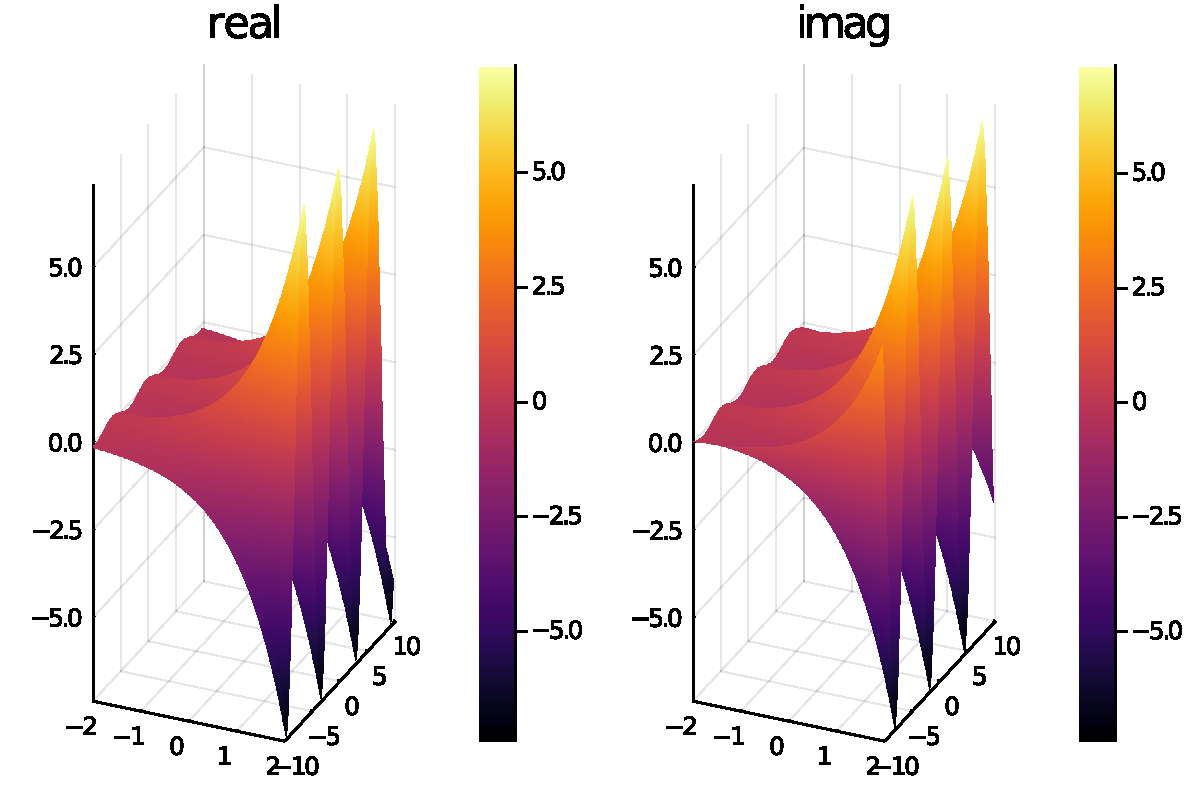
\includegraphics[width=\linewidth]{figures/Lecture0_3_1.pdf}

You can also include text and LaTeX code in Jupyter notebooks. Alternatives to Jupyter notebooks include \href{https://junolab.org/}{Juno} and \href{https://github.com/fonsp/Pluto.jl}{Pluto}.



\end{document}
